\section{System design}
I dette afsnit vil koncepterne bag mange af de teknologier, der gør systemet muligt, blive belyst, men der vil også blive analyseret og diskuteret, hvordan systemet skal designes. Dette vil blive gjort ud fra hvordan kravspecifikationen best muligt vil blive opfyldt.
Systemet bliver gennem kravspecifikationen pålagt både at være sikkert, men samtidig også at skulle køre med en fornuftig indlæsnings tid. Disse krav modarbejder for det meste hinanden på flere forskellige måder, og er derfor relevante for forståelsen af processen der leder op til det endelige system. Systemet er beskrevet generelt i afsnit \ref{produkt_beskrivelse} og senere i afsnit \ref{Opsummering_Overvejelserne}. 

\subsection{Central eller decentral løsning}
%Hvad er centraliceret system / decentraliceret
Løbende opdateringer, til et system for hemmelige beskeder over sociale medier, menes essentielle. F.eks. kunne de enkelte sociale medier til enhver tid nedlægge et sådan hemmeligt systems anvendte konti-bots, eller selve dets sociale netværk kunne ændre sin struktur fra en dag til den næste.
% Centraliceret bot information
I dette system anvendes f.eks. flere dynamisk generede bots, til at sikre brugerens anonymitet, samt også til deres generelle kommunikation på platformen. Men grundet at de sociale medier generelt ikke ønsker systematisk genererede anonyme brugere på deres platform, og at disse bots desuden også kunne være associeret med en potentielt mistænkelig opførelse, vil en opdateret information om disse anvendte bots findes nødvendig.
% Opdaterings mulighed
Et centraliseret system åbner muligheden for dette, da et sådant system altid kan opdateres løbende, hvilket findes mere besværligt i et decentraliseret system. I et decentraliseret system kunne forskellige brugere, under et dynamisk udviklende miljø, nemlig ende med at være fastlåst med software, der potentielt er defekt, eller ville kræve at blive hentet på ny.
En sådan mulighed for løbende opdateringer, anses også mange gange for essentiel under en mulig skalering af systemer, blandt andet når systemets behov kræver større fundamentale re-designs, og er derfor ofte anvendt.
% Fokus på køretid
For dette projekts syn vil et større centraliseret system også anses for at være favorabelt, da dette potentielt vil øge hastighed ved brugerenes anvendelse. F.eks. kunne en centraliseret server indeholde en kortlægning af alle relevante opslag, og derved mindske de enkelte brugeres søgninger, eller mindske antallet af påkrævede anmodninger til de forskellige sociale medier.
% Fokus på sikkerhed 
Til gengæld, for samme i et decentraliseret system, kan en centrale server nemt spærres fra en tredjepart, og ville derfor være et vigtigt knudepunkt i systemet.

\begin{figure}[H]
    \begin{subfigure}{0.5\textwidth}
        \centering
        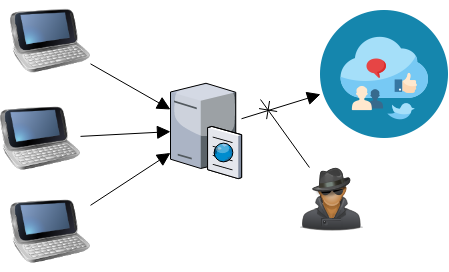
\includegraphics[width=1\linewidth, height=4cm]{Projectdoc/Assets/Illustrationer/Security_diagram_1.png} 
        \caption{Central server}
        \label{fig:central_server}
    \end{subfigure}
    \begin{subfigure}{0.5\textwidth}
        \centering
        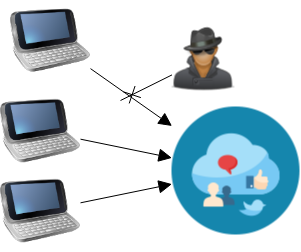
\includegraphics[width=0.7\linewidth, height=4cm]{Projectdoc/Assets/Illustrationer/Security_diagram_2.png}
        \caption{Klient-baseret system (decentral)}
        \label{fig:decentral_server}
    \end{subfigure}
    \caption{Forskellen på central og decentral server struktur}
    \label{fig:serverstruktur}
\end{figure}

Hvis projektet i stedet for hastighed skulle anse højere sikkerhed, ville et decentraliseret system, potentielt være at foretrække. 
Et decentraliseret system indeholder nemlig nødvendigvis ingen knudepunkter [Figur \ref{central_server}], og et eventuelt system nedbrud eller informations lækage, ville derfor være mindsket, da der ikke findes et centralt brist.
Selvfølgelig ville enkelte del punkter, stadig have mulighed for at blive blokeret, men i sådanne tilfælde ville dette, kontra i et centraliseret system, ofte ikke blokere nogen større helhed [Figur \ref{fig:decentral_server}].
% Største centraliserings metode
Et centraliseret system kan dog stadig sikres yderligere. F.eks. kunne tilgangen fra de enkelte brugeres enheder mindskes ved opsætning af en større database, med formålet udelukkende at indeholde information om mindre servere, der potentielt kunne indeholde mindre grupperinger, med informationen for de anvendte bots. Derved mindskes opmærksomheden på systemets centrale knudepunkt, da denne kun findes nødvendig at kontakte, hvis forbindelsen til de mindre ikke kan etableres, f.eks. ved blokering af disse. Denne struktur ville også mindske faren ved potentiel overvågning, da lækagen kun ville være gældende for de mindre partioner af systemet.
Samme funktionalitet kan selvfølgelig også opnås gennem et decentraliceret system, hvis man i stedet for at anvende en større server, opdaterede de enkelte klienter igennem system opdateringer. Til gengæld vil dette øge de enkeltes mulighed for fejl, men man ville herved ikke kræve samme vedligeholdelse og hardware specifikationer.
% Kryptering





%\section{System design}
%I dette afsnit vil det blive analyseret og diskuteret hvordan systemet skal designes, ud fra hvordan kravspecifikationen bedst muligt vil blive opfyldt. Koncepterne bag mange af de teknologier, der gør systemet muligt vil også blive belyst. Problematikkerne samt dilemmaerne, som rejser sig under system designs processen skaber strukturen i afsnittet, og leder op imod det samlede forslag til et system.

\subsection{Central eller decentral løsning}
Ud fra kravspecifikationen bliver systemet pålagt at være sikkert, men samtidig også at køre med en fornuftig indlæsnings tid. Disse krav kan modarbejde hinanden på flere forskellige måder, blandt andet i spørgsmålet om, om systemet skal køre centralt eller decentralt.
\\\\
Hvis man har spørgsmålet med optimal indlæsnings tid i mente, vil en central løsning med en server der lagrer stien til alle beskeder i systemet være favorabel. Dette gør enheder der tilgår den centrale database i stand til at forespørge og efterfølgende finde opslag meget hurtigt, da databasen har kortlagt alle relevante opslag. Dette står i modsætning til en decentral løsning, hvor brugernes enhed selv skal søge efter de relevante opslag. Den søgning kræver samtlige server anmodninger på hvert enkelt enhed, da den centrale kortlægning ikke er tilgængelig. De mange anmodninger vil resultere i længere indlæsnings tid.

%Før værende billede sikkerhed

En central server trods dens eventuelle positive egenskaber, kan dog også udgøre et sikkerhedshul, hvis denne server ikke er sikret tilstrækkeligt. Med andre ord lægger dette en systemvedligeholdelses byrde på dem der administrerer systemet. F.eks. kunne en sådan server, (Illustreret ved [Figur \ref{fig:central_server}]), lække generelle lagerede informationer, eller ligefrem blive overvåget for kommunikation, samt blive spærret som en helhed. Dette vil selvfølgelig også kunne ske for den enkelte bruger [Figur \ref{fig:decentral_server}], men disse blokeringer ville i sådanne tilfælde også kun påvirke den enkelte, og ikke systemet som en helhed.
Hermed har begge løsninger gode og dårlige elementer. Derfor vil forskellige aspekter af kommunikationsplatformen blive videre diskuteret for at kunne finde et kompromis mellem helt centraliseret og helt decentraliseret.

%Før værende billede sikkerhed
\begin{figure}[H]
    \begin{subfigure}{0.33\textwidth}
        \centering
        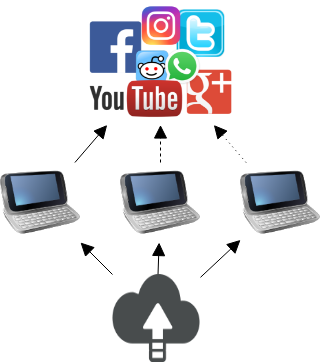
\includegraphics[width=0.7\linewidth, height=4cm]{Projectdoc/Assets/Illustrationer/Device_Opdate.png} 
        \caption{Lokale enheds kendte lister, opdateret via softwareopdateringer}
        \label{fig:DeviceOpdate}
    \end{subfigure}
    \begin{subfigure}{0.33\textwidth}
        \centering
        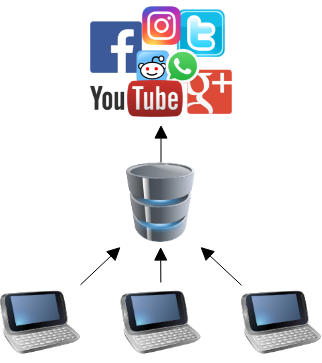
\includegraphics[width=0.7\linewidth, height=4cm]{Projectdoc/Assets/Illustrationer/CentralDatabase.png}
        \caption{Én central database}
        \label{fig:CentralDatabaseList}
    \end{subfigure}
    \begin{subfigure}{0.33\textwidth}
        \centering
        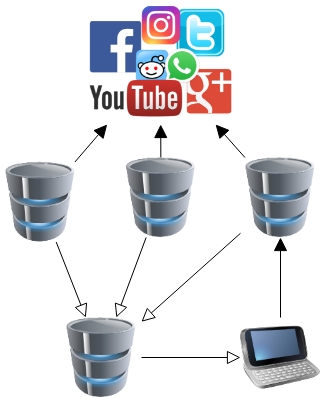
\includegraphics[width=0.7\linewidth, height=4cm]{Projectdoc/Assets/Illustrationer/MainDomainServer.png}
        \caption{Et netværk af databaser, kendt af enhederne, og opdateret fra en hoveddatabase}
        \label{fig:MainDomain}
    \end{subfigure}
    \caption{Forskellige medie kontakt former.}
    \label{fig:MedieContact}
\end{figure}

For at kunne opretholde en mængde af bots, her forstået som anonyme brugere på sociale medier genereret af systemet, der har til opgave at sikre anonymitet for brugeren på kommunikationsplatformen, vil det være nødvendigt at kunne tilføje nye bots til netværket løbende, samt opdatere status af nuværende bots. Dette er nødvendigt da det kunne formodes at ejerne af det relevante sociale medie ikke ønsker systematisk genereret anonyme brugere på deres platform, specielt hvis de er associeret med en potentielt mistænkelig opførelse. 
% 
For at systemet kan fungere, skal systemet vide hvilke bots der er tilgængelige på et hvert tidspunkt. Én mulig måde at holde styr på disse informationer kunne være, som illustreret ved [Figur \ref{fig:CentralDatabaseList}], en database opdateret med information om de enkelte bots på de sociale medier. Databasen kan lagre om de stadigvæk er aktive, eller om de er blevet banlyst af det sociale medie, f.eks. for ikke at være en "normal" bruger. Hvis en given bot så blev lukket ned, ville den opdaterede database, gøre enhver bruger i stand til blot at vælge en anden bot. Denne løsning tilfører dog et element, en database, som vil være et kritisk led for, at tilbyde yderligere anonymitet til brugeren. Hvis denne database så ikke er tilgængelig, vil denne funktionalitet være hindret, i det at bots vil kunne blive taget ned i mellemtiden, uden at brugeren ville vide det, da dette sker før brugeren får en fejlmeddelelse.\\ 
Et værre scenarie forestilles ved kompromitteringen af denne database, der vil gøre det muligt for uvedkommende at læse beskederne sendt igennem systemet. Dette scenarie vil især være vigtigt for sikkerheden, hvis der er anvendt kryptering af beskedernes tekst, som en ekstra form for sikkerhed. Disse krypteringsnøgler vil i sådanne tilfælde skulle gemmes et sikkert sted, uden denne fare for kompromittering, men stadig et sted hvor alle de egentlige bruger kan få fat i dem.\\ 
En måde hvorpå man kunne sikre systemet under en central server, er ved at holde sammenkædningsfunktionaliteten på serveren. Hvis serveren så ikke er tilgængelig, vil det være meget tidskrævende at finde de billeder som indeholder beskederne, da billederne som. Efter disse billeder så er fundet, vil det så også kræve krypteringsnøglerne som kunne være gemt i kildekoden. På denne måde kunne en central servers nedbrud hindre brugere, såvel som uvedkommende, i at tilgå beskederne i systemet.

Som løsning på dette, kunne man opstille databasen, så den kun kontaktes af brugerne der skal opdatere deres bot informations liste. Dette vil mindske trafikken imellem databasen og klienterne, og derved vil dens opmærksomhed være mindre.\\
% 
Man kunne også forestille sig en ekstra database, som illustreret ved [Figur \ref{fig:MainDomain}], der kun vil blive kontaktet hvis den primære er inaktiv, og at denne database kender til andre databaser, der opererer som backups af den primære. Denne opbygning vil gøre det meget svært at lukke systemet i længere tid. På den anden side vil denne opsætning også kræve mere hardware og mere vedligehold i form af synkronisering, opdatering osv. Dermed vil en opsætning af en sådan backup koste systemadministratoren mere arbejdstid, og vil derfor kræve en vurdering af, om opsætningen er investeringen værd.\\
% 
En måde at undgå dette databaseproblem, er at lade hver klient have en lokal liste over aktive bots, som illustreret ved [Figur \ref{fig:DeviceOpdate}]. Denne liste vil så med jævne intervaller blive opdateret igennem klient opdateringer. Med denne fremgang er det tænkeligt, at systemet vil kræve mange opdateringer, eller at der ofte vil være et antal utilgængelige bots på listen, i denne illustration vist ved de stiplede linjer.
\\\\
Som førnævnt vil et centraliseret system betyde at hele systemet vil hvile på en node, hvilket vil betyde at en angriber blot skal tage et led ud for at kollapse hele systemet. 
En måde hvorpå man kunne sikre systemet under en central server, er ved at holde sammenkædningsfunktionaliteten på serveren. Hvis serveren så ikke er tilgængelig, vil det være meget tidskrævende at finde de billeder som indeholder beskederne. Efter disse billeder så er fundet, vil det så også kræve krypteringsnøglerne som kunne være gemt i kildekoden. På denne måde kunne en central servers nedbrud hindre brugere, såvel som uvedkommende, i at tilgå beskederne i systemet. lagre krypteringsnøgler på serveren, der skal hentes for at kunne læse en besked. Denne centrale server bliver det eneste led som en ondsindet angriber skal lægge ned, for at gøre hele platformen ubrugelig. Dette vil faktisk sikre brugerne, såfremt angriberen ikke kompromitterer krypteringsnøglerne. Brugernes beskeder vil være ulæselige for en angriber uden de krypteringsnøgler. Dette kan sammenlignes med en indbygget selvdestruktion af systemet.\\
Et centraliseret system kan altså altid opdateres løbende, i modsætning til den decentraliseret løsning hvor brugerne enten er fastlåst med software der potentielt er defekt eller skal hentes på ny. Løbende opdateringer til systemet er essentielle når det sociale netværks bot konti, ikke fungerer som tiltænkt. Dette kan ske på mange forskellige måder: Blandt andet kan de enkelte bots blive taget ned for mistanke for falsk bruger, eller netværket kunne ændre sin struktur fra en ene dag til den anden. Muligheden for løbende opdatering er også essentiel ved en mulig skalering af systemet, blandt andet når systemets netværk af bots ikke kan betjene en voksende brugerbase, eller når denne brugerbase ændrer behov der kræver at det fundamentale system gennemgår strukturel redesign.
\\\\
\textbf{Samlet løsning}\\
Selvom en komplet decentraliseret løsning lyder godt på papiret, så vil det udløse så mange fundamentale problemer at systemet vil være bøvlet og potentielt ubrugeligt. Da systemet afhænger så kraftigt af en trejdeparts service, så vil små ændringer, så som disse, gøre systemet ubrugeligt:
\begin{itemize}
    \item[-] Systemets bot netværk kan blive delvist eller helt lukket ned. Dette kan ske af mange forskellige grunde blandt andet ved brud på det sociale medies ToS (Terms of Service) eller ved en eventuel afsløring af hele systemet / projektet. 
    \item[-] Tredjeparten kan ændre deres API struktur på sådan vis at det fundamentale system ikke længere fungerer som tiltænkt.
\end{itemize}

\subsection{Sammenkædning af beskederne}
På projektets sikrede kommunikationsplatform vil det være nødvendigt at kunne finde sammenhængende beskeder, samtidig med at denne sammenkædning vil ikke kunne foregå på åbenlys vis på et socialt medie. I stedet kunne én mulighed være, at gemme sammenhængen i noget tilsyneladende uskyldig metadata, men som er genereret ud fra en prædefineret algoritme. Dette vil give den sikrede kommunikationsplatform noget specifikt at søge efter, uden at det vil være et let læseligt flag. Men hvad er metadata?

\subsubsection{Metadata}
Metadata kan grundlæggende defineres som data om data. Dermed kan det anvendes i mange sammenhænge. Et eksempel kunne være et billede. Dataen i et billede er i simpleste forstand lysintensiteter, i sort/hvid billeder, eller farver. Men udover denne data kunne man også gemme ting som dato, klokkeslet, GPS koordinater, navnet på ophavsmanden osv. Alt dette er eksempler på metadata som ikke påvirker indholdet, men som gør indholdet mere brugbart i mange forskellige sammenhænge. For eksempel vil vedhæftede søgeord gøre et billede galleri meget mere effektivt i at præsentere det ønskede materiale. Metadata kan både genereres automatisk af hardware/software systemer, men en bruger kunne også tilføre metadata manuelt.\\ 
% Giv billede eksempler på meta på sociale medier (måske)
\begin{table}[H]
    \begin{minipage}{.65\textwidth}
        \begin{figure}[H]
        \centering
        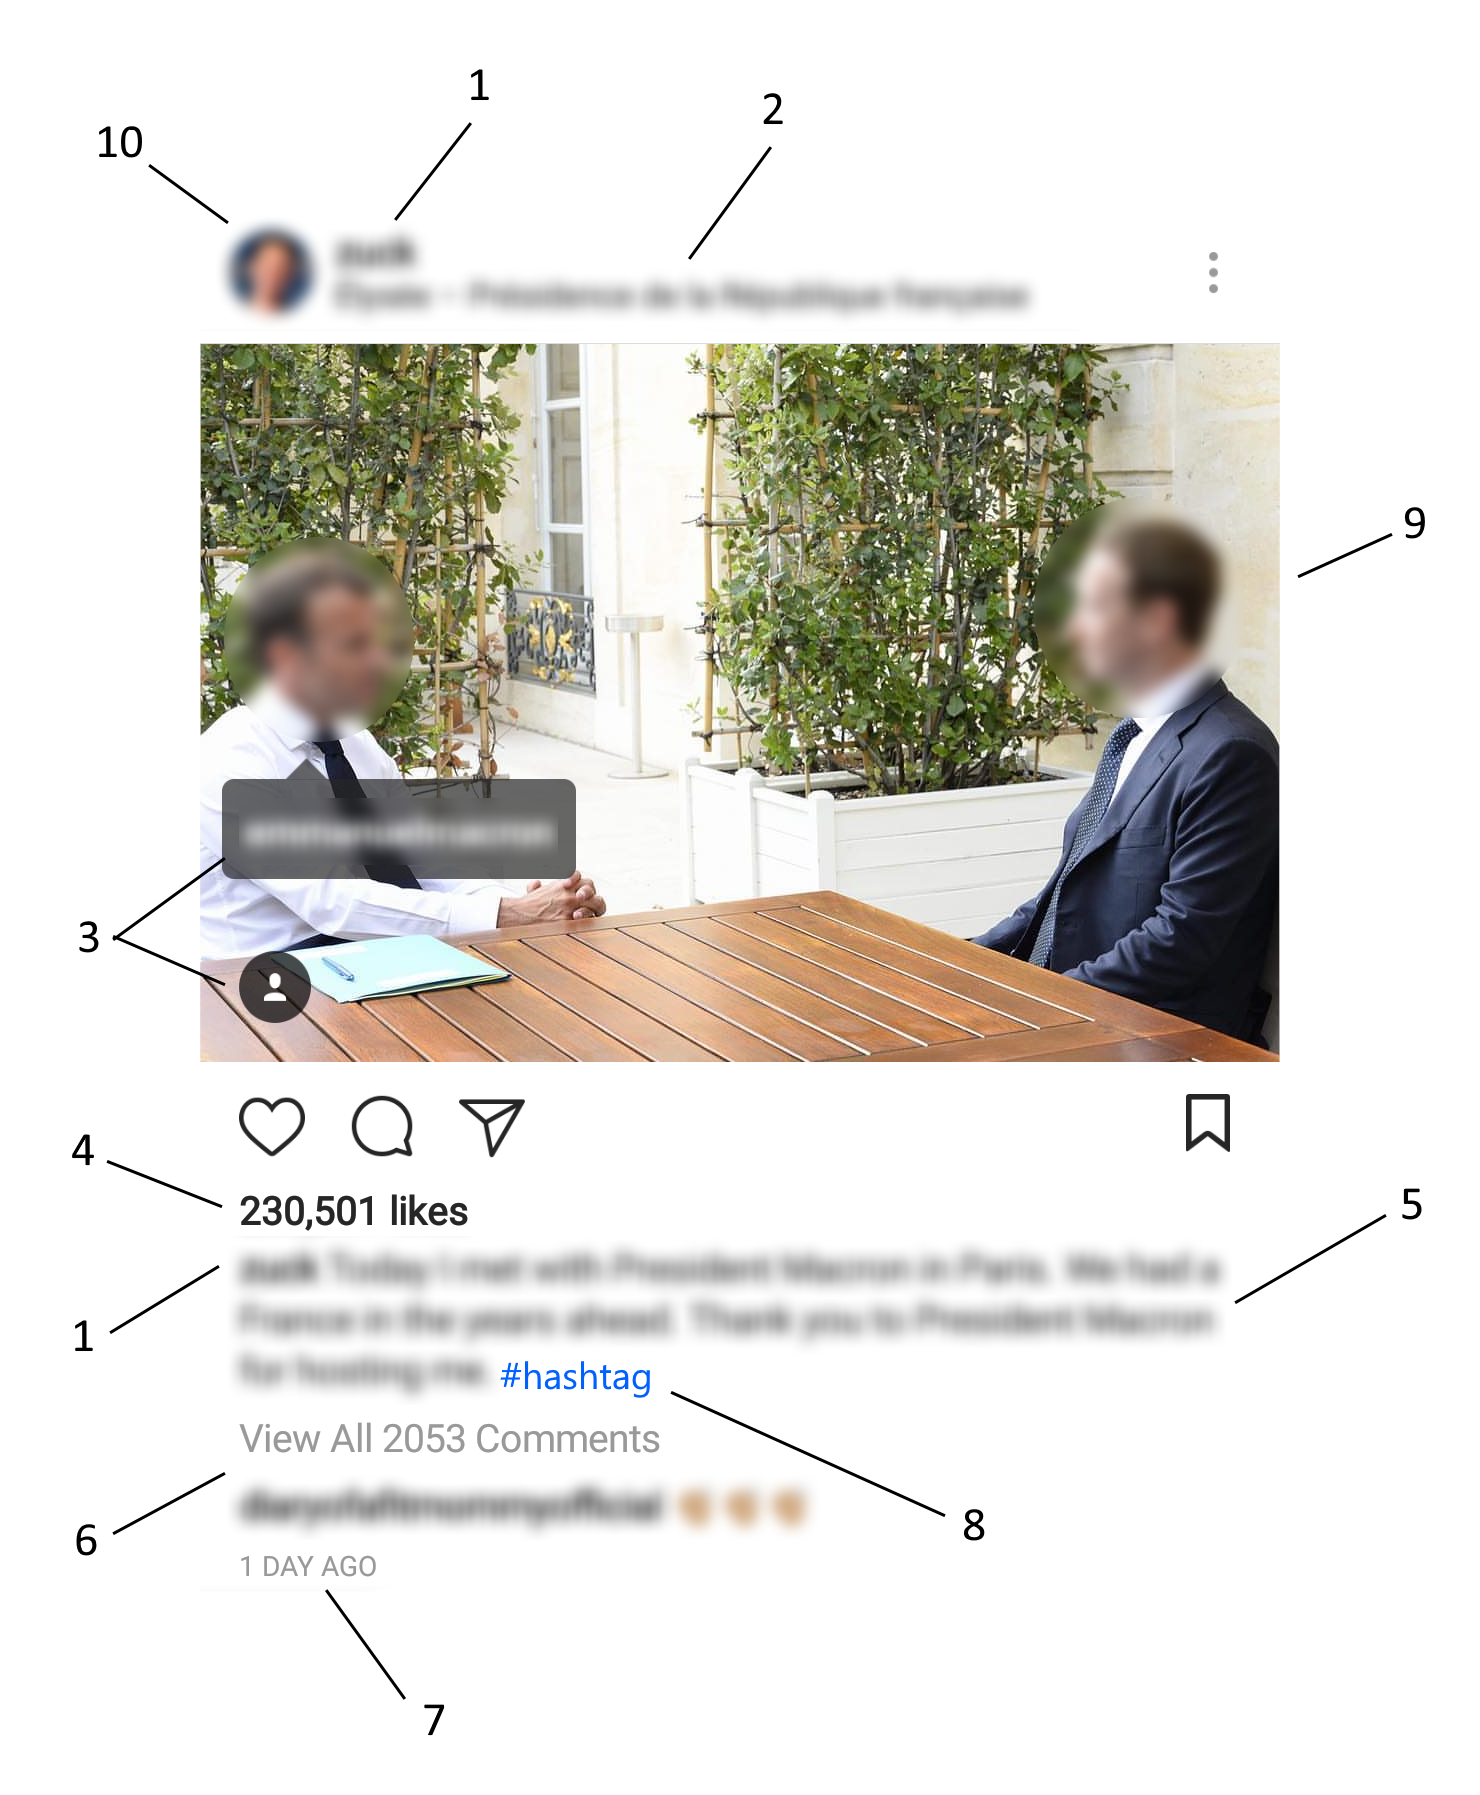
\includegraphics[width=1.0\linewidth ]{Projectdoc/Assets/Illustrationer/IG-meta.png} 
        \caption{Stackoverflows forum struktur YOLO}
        \label{fig:ig_metadata}
        \end{figure}
    \end{minipage}
    \begin{minipage}{.35\textwidth}
        \begin{enumerate}
            \item Brugernavn
            \item Lokation
            \item 3
            \item 4
            \item Beskrivelse
            \item Kommentarer
            \item Klokkeslet
            \item Hashtags (Kategorisering)
            \item Billedet
            \item Profil billede
        \end{enumerate}
    \end{minipage}
\end{table}

Dette er især sandt på sociale medier hvor der kan findes en stor mængde af generelle søgeord. Netop det faktum at sociale medier tillader de enkelte brugere at skabe en varierende mængde af metadata for et hvert billede, sandsynliggør at systemet vil være i stand til at generere disse søgeord med en prædefineret algoritme for hver tråd på forummet. Dette vil så gøre det muligt at søge efter nye opslag på enhver forumstråd.

\subsubsection{Forum struktur}
Da et forum kan designes på flere måder vil det her blive diskuteret hvilken struktur der vil passe bedst til produktets tænkte anvendelse. Som det kan ses i [Figur \ref{fig:forskellige_fora}] er både Stackoverflow og Jodel fora, men med vidt forskellige formål. Stackoverflow er generelt set anvendt til at løse specifikke problemer. Disse problemer kan så gives relevante søgeord og kan på den måde opdages af interesserede personer. Der er også kategorier som samler de nyeste opslag eller mest sete osv.

\begin{figure}[H]
    \begin{subfigure}{0.5\textwidth}
        \centering
        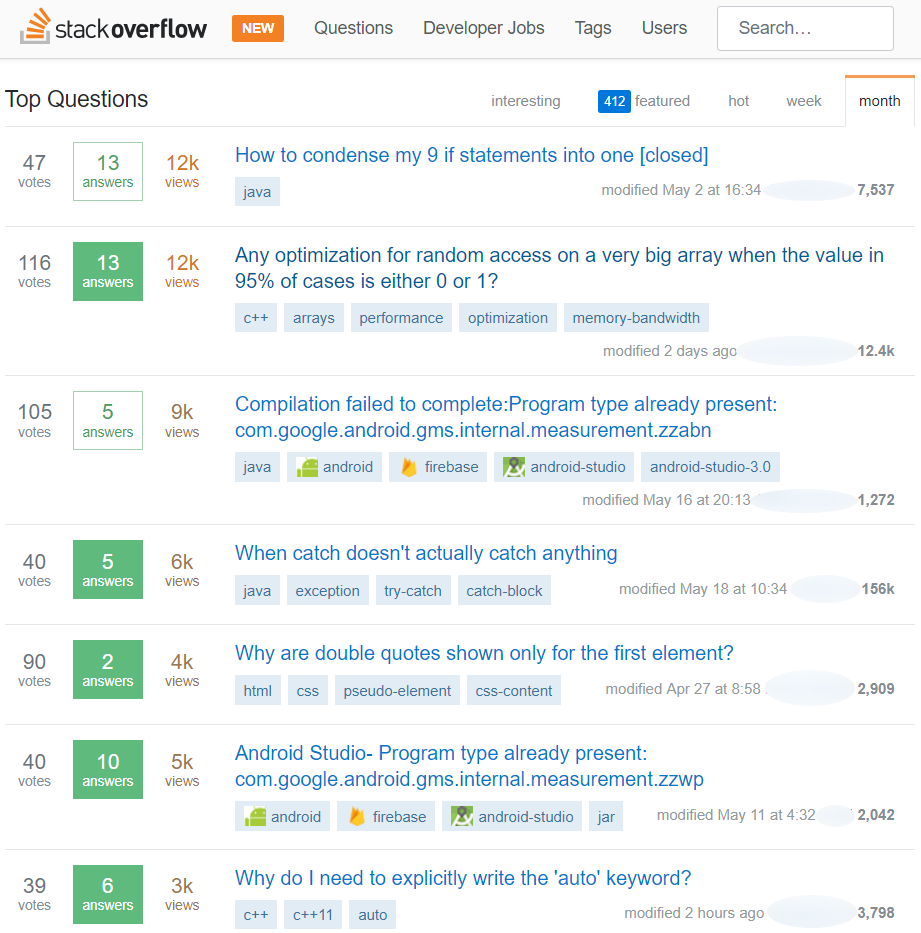
\includegraphics[width=1.0\linewidth ]{Projectdoc/Assets/Illustrationer/stackoverflow_forum_eksempel.png} 
        \caption{Stackoverflows forum struktur}
        \label{fig:stackoverflow_forum}
    \end{subfigure}
    \begin{subfigure}{0.5\textwidth}
        \centering
        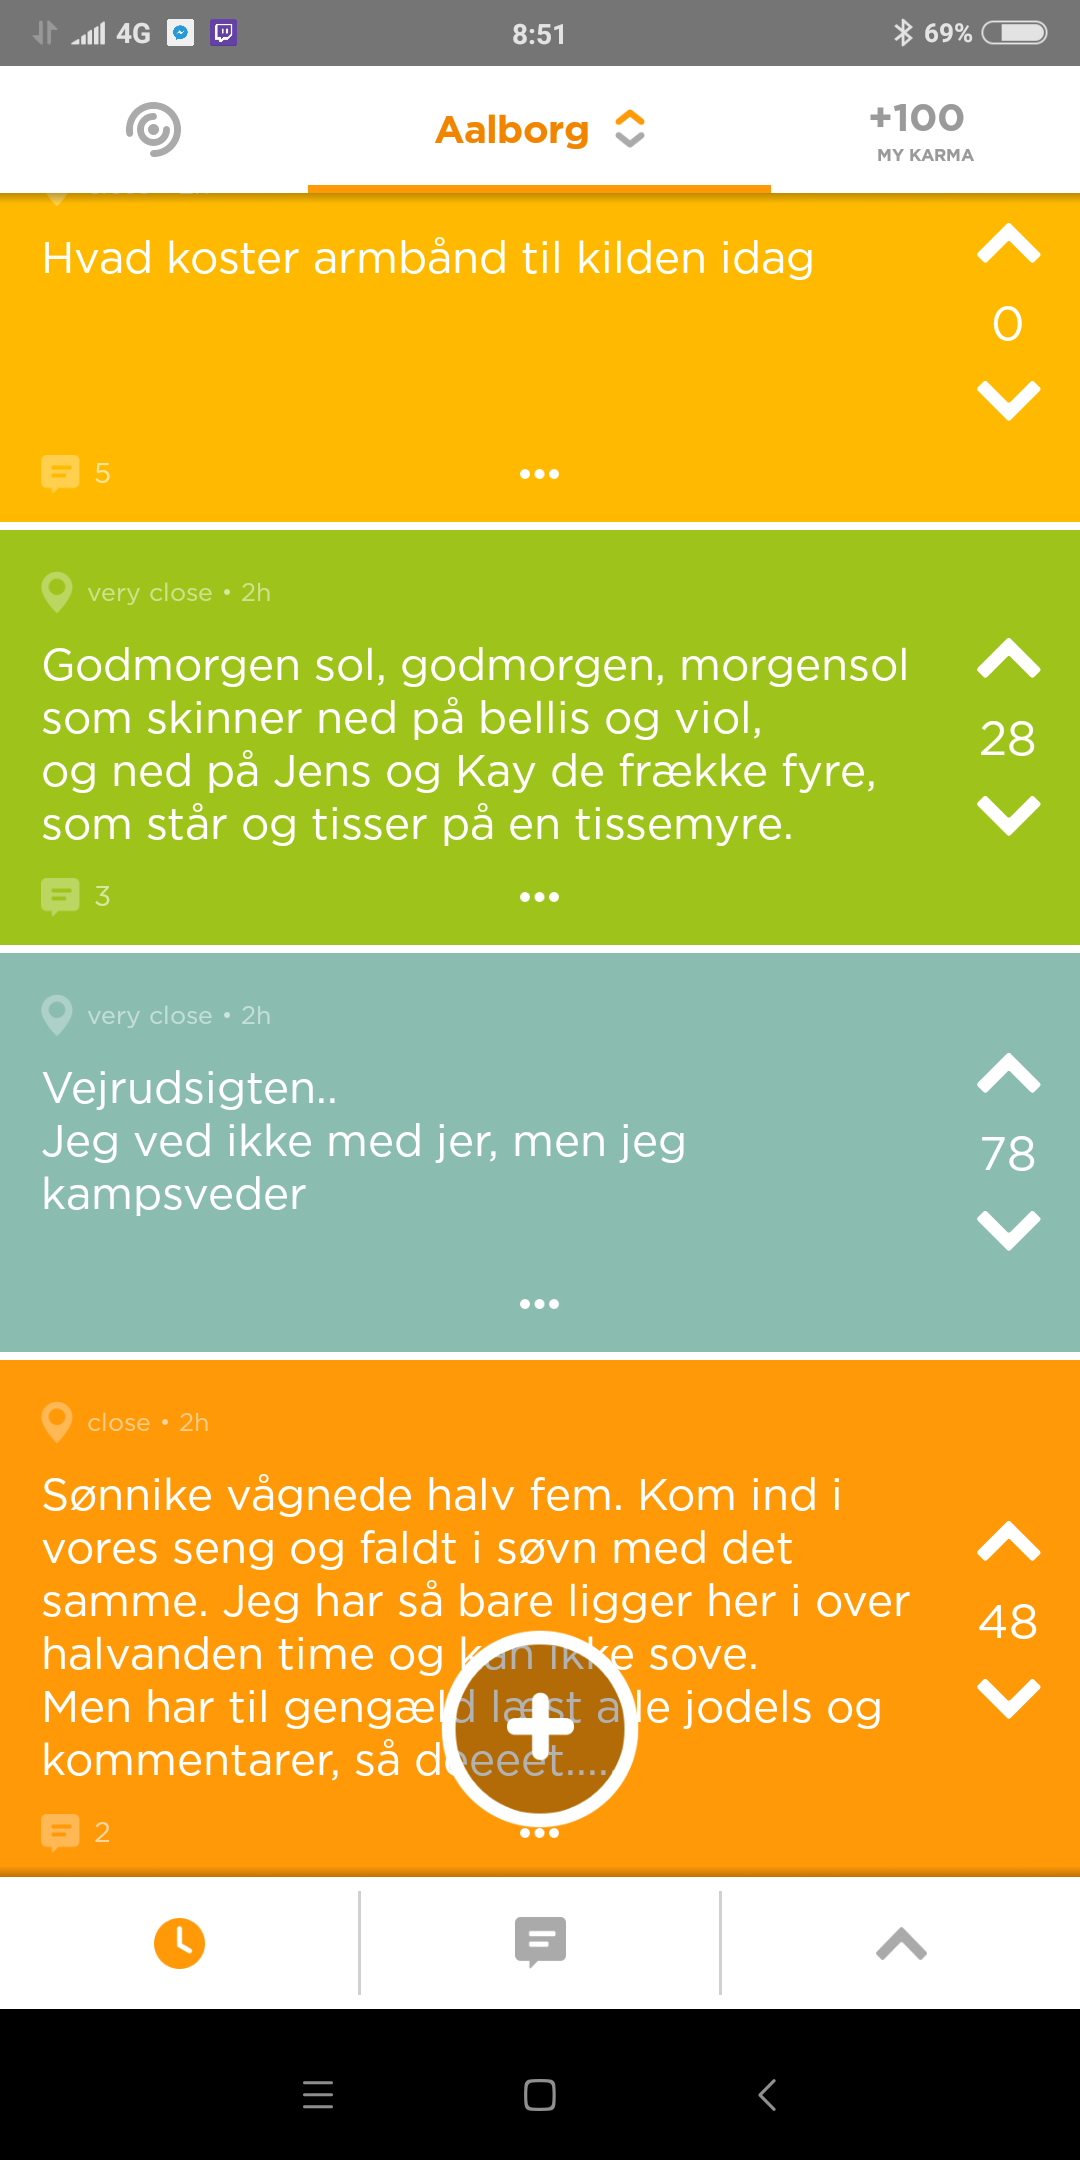
\includegraphics[width=0.7\linewidth]{Projectdoc/Assets/Illustrationer/jodel_forum_eksempel.png}
        \caption{Jodels forum struktur}
        \label{fig:jodel_forum}
    \end{subfigure}
    \caption{Forskellige fora}
    \label{fig:forskellige_fora}
\end{figure}

I kontrast til dette er Jodel en mere ufiltreret, og tilfældig, samling af anonyme opslag. Det eneste der er fælles for opslagene man ser på Jodel er, at de er inden for en bestemt fysisk radius af hinanden.
Da systemet gerne skulle kunne bruges til seriøse diskussioner om vigtige emner, så virker noget ligende Stackoverflows model som en god idé. Man kunne også forestille sig et "lokalt" feed som kunne medføre lokations specifikke diskussioner.\\
Hvis disse to funktionaliteter ønskes, vil det kræve to forskellige sammenkædnings algoritmer, da den ene er baseret på lokation og den anden på tråd. Dette vil give anledning til to potentielt meget forskellige køretider. Dette vil det næste afsnit bearbejde.

\subsubsection{Forespørgsler og køretid}
Køretiden på systemets forespørgsler afhænger af flere faktorer: Mængden af de forespørgsler systemet laver til det sociale medie, tiden det tager at behandle den modtaget data samt trejdepartens systems køretid. Den sidstnævnte er uafhængig af systemet selv og kan derfor ikke optimeres. Det kan forespørgsels algoritmen og behandlingsprocessen af besked udvindingen. 

% Wrap figure
\begin{figure}[H]
    \centering
    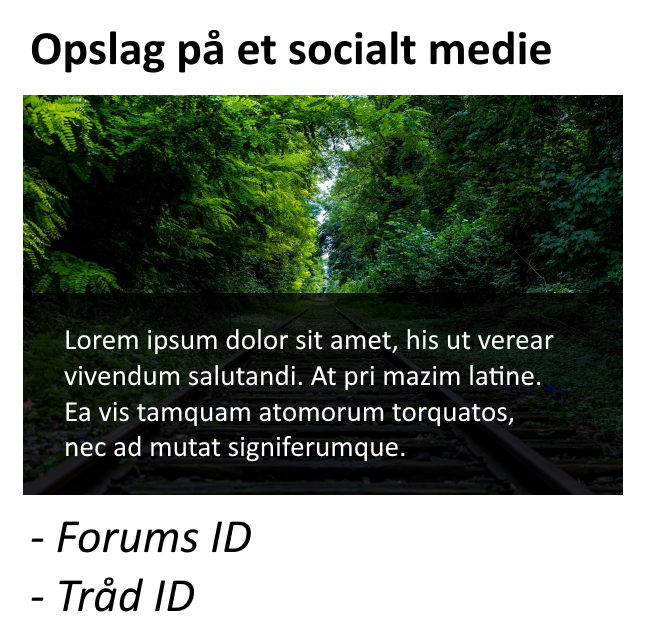
\includegraphics[width=0.5\linewidth]{Projectdoc/Assets/Illustrationer/requests.png}
    \caption{}
    \label{fig:køretid}
\end{figure}

Når en bruger af systemet vil navigere til et specifikt forum, så vil der blive sendt en forespørgelse til alle de relevante bots der lagre opslag. Systemet søger nu efter et specifikt stykke metadata, som kun systemet vil kunne genkende, men som uvidende personer ikke med det blotte øje kan tyde. Det første stykke information systemet leder efter er et \textit{forum ID} der henter alle opslag tilknyttet det ønskede forum. Det har potentiale til at være rigtig mange forespørgelser for at genere en forumsoversigt. Systemet kigger derfor også ikke et \textit{tråd ID} som bruges t

% Forklar hvordan vores valgt af løsning virker på algoritmen
% - Hvordan kan man sikre en fornuftig køre tid? (Undg̊a 10000 undersøgelser for at finde  ́en kommentar)
% - Formindsk chancen for mistænkelig data trafik. Både i server requests og det visuelt uploaded

\subsubsection{Private beskeder (Brug af unikt hash)}
En feature der vil kunne tilbyde yderligere sikkerhed for bestemte typer af brugere og brugsmål er muligheden for at sende private beskeder. For at kunne tillade brugere at kommunikere privat til hinanden, er en unik identifikations bestemmelse for begge brugere strengt nødvendigt. Systemet kan derfor ikke tildele en offentlig bot konto for denne aktivitet, da det ikke er realistisk for systemet at tilegne en unik bot til hver bruger af systemet.\\
For at en feature som denne kan realiseres, vil det kræve at brugeren selv opretter eller tilknytter sin konto fra det pågældende sociale medie. Det giver systemet adgang til at lagre den hemmelige besked på brugerens konto, hvor kontoens unikke bruger ID fra det sociale medies database nu kan bruges til identifikations bestemmelse. Systemet anvender bruger ID i en hashing algoritme til at genere en, for systemet, læsbar adresse som der kan deles indbyrdes mellem de der ønsker at sende privat til hinanden. Kun systemet kan oprette og genkende disse hash-koder, som der kan samles for at danne en privat gruppechat. Denne hash genkendelse kunne også udvides til at supportere flere forskellige sociale netværk ad gangen, såfremt at systemet har en metode til at kende forskel på diverse sociale netværk.
\\\\
\textbf{Brug af brugerkonti i hele systemet}\\
Et system baseret på brugernes login i samarbejde med system kontrollerede konti, har også været en overvejelse. Systemet går ud på at brugeren opretter forum opslag fra systemet, der ligger den hemmelige besked i et billede på brugerens egen profil. Problemet ved dette er dog at det krævede dobbelt arbejde fra systemet, da systems bots kun holder styr på beskedens lokation. Det vil sige at systemet først skal sende en forespørgelse til alle de aktive bots, som så forespørger den enkelte brugers profil. Et af fordelene var dog at systemet kunne kæde brugerne sammen med de opslag de lavede, selvføjelig med et anonymiserende hash. Det kasserede system er beskrevet yderligere i appendix \ref{userbased}.

\subsection{Opsummering af alle overvejelserne}
\label{Opsummering_Overvejelserne}
Ud fra de overstående overvejelser og metoder, kan et endeligt system dannes som følgende struktur:

\begin{figure}[H]
    \centering
    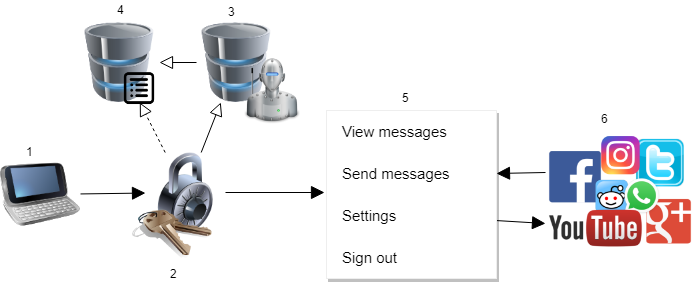
\includegraphics[width=0.70\linewidth]{Projectdoc/Assets/Illustrationer/System_struckure.png}
    \caption{System}
    \label{fig:sysdiagram}
\end{figure}

Systemets struktur beskriver, en central database [Figur \ref{fig:sysdiagram}.4] indeholdende information om alle systemets mindre databaser [Figur \ref{fig:sysdiagram}.3], der kan eksistere i uvist eller dynamisk antal, og videre indeholder informationer til anonyme brugere, om de aktive bots, der er dynamisk genereret til de enkelte sociale medier.\\
Denne centrale database er herved kun tilgået fra slutenhederne, når de ikke længere kan tilgå enkelte mindre databaser, symboliseret [i Figur \ref{fig:sysdiagram}.2, \ref{fig:sysdiagram}.3 og \ref{fig:sysdiagram}.4] med en stiplet linje, og har derfor ingen direkte forbindelse til omverdenen, ud over de enkelte enheder.\\
Den centrale database kræver kun vedligeholdelse af dens indhold, men til gengæld kræver de mindre databaser opsætning for hver gang de opdateres og efter eventuelle lukninger fra sociale medier. Her vil de falske konti selv også kræve det samme.
Enhederne [Figur \ref{fig:sysdiagram}.1] kan herefter selv hente information, fra disse mindre databaser, nødvendigt for at danne beskederne, og til sidst også selv poste eller hente beskeder, samt besked tråde, til og fra de sociale medier.

% Ref til talve skitse: \ref{appendix:earlysystem}